\documentclass[10pt]{article}

\usepackage[a4paper,margin=0.65in]{geometry}
\usepackage[utf8]{inputenc}
\usepackage{graphicx}
\usepackage{titlesec}
\usepackage{fancyhdr}
\usepackage{color}
\usepackage{parskip}
\usepackage{helvet}
\usepackage{longtable}
\usepackage{hyperref}
\usepackage{float}
\usepackage{caption}
\usepackage{lastpage}
\usepackage{array}
\usepackage{ragged2e}
\usepackage{makecell}
\usepackage{tabularx}
\usepackage[table]{xcolor}
\usepackage{colortbl}
\usepackage{placeins} % para FloatBarrier

% Colores para tablas
\definecolor{headergray}{gray}{0.9}
\definecolor{rowalt}{RGB}{245,245,255}

% Fuente sans-serif
\renewcommand{\familydefault}{\sfdefault}

% Encabezado
\pagestyle{fancy}
\fancyhf{}
\lhead{
\includegraphics[height=0.7cm]{images/logo_unit.png}}
\rhead{\textbf{UNIT Magnetometer BMM150 Module v1.0}}
\lfoot{Product Brief}
\rfoot{\thepage\ | \pageref{LastPage}}

% Estilo de secciones
\titleformat{\section}{\bfseries\large\sffamily}{}{0em}{}
\titleformat{\subsection}{\bfseries\normalsize\sffamily}{}{0em}{}
\titlespacing*{\section}{0pt}{1.2em}{0.5em}
\titlespacing*{\subsection}{0pt}{0.8em}{0.4em}

\title{}
\author{}
\date{}

\sloppy
\setlength{\emergencystretch}{3em}

\begin{document}

% Encabezado del documento
\noindent
\makebox[\textwidth][l]{%
    \begin{minipage}[t]{\textwidth}
        \Large \textbf{UNIT Magnetometer BMM150 Module Product Brief}\\[1.0em]
        \normalsize A passive buzzer module is a sound-generating device that produces tones when controlled by a PWM signal from a microcontroller.\\[0.3em]
        \footnotesize\textsf{Version: 1.0 \hfill Modified: 2025-05-19}
    \end{minipage}%
}
\vspace{1em}
\hrule
\vspace{1.5em}

% Introducción con imagen
\section*{Introduction}
\vspace{0.5em}
\noindent
\begin{minipage}[t]{0.62\textwidth}
\setlength{\parskip}{0.75em}
\justifying
The BMM150 is a compact, ultra-low-power 3-axis digital magnetometer designed for precise magnetic field sensing. It is ideal for applications such as electronic compasses, inertial navigation, and orientation detection in embedded systems. Supporting both I²C and SPI interfaces, the BMM150 integrates easily with popular microcontrollers like Arduino, ESP32, and Raspberry Pi. Its efficient power consumption and robust performance make it an excellent choice for portable devices, IoT projects, and wearable technology.
\end{minipage}
\hfill
\begin{minipage}[t]{0.35\textwidth}
\centering
\vspace{-0.5em}
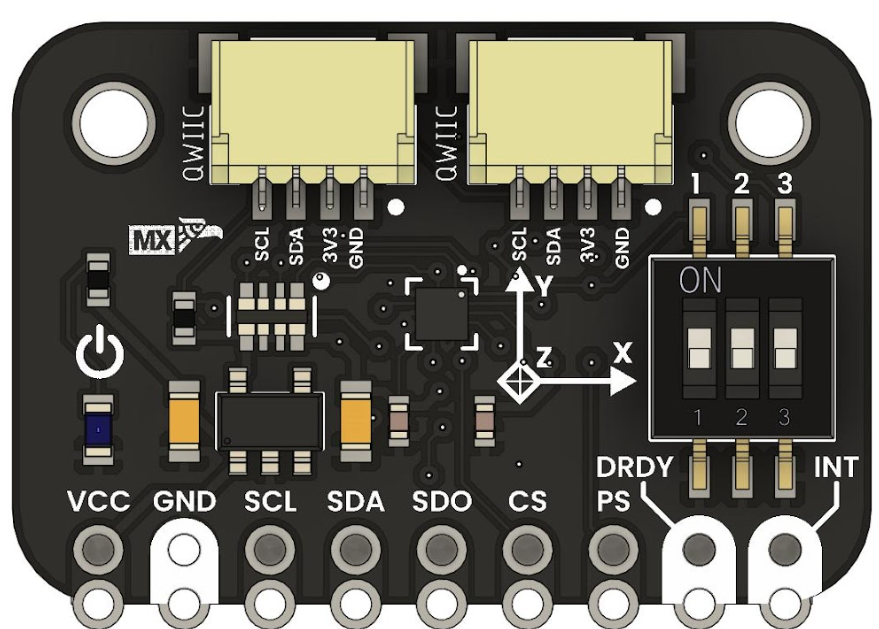
\includegraphics[height=3.5cm,keepaspectratio]{./images/product.png}
\end{minipage}

\vspace{1.0em}
\FloatBarrier % evita que la imagen flote sobre el siguiente bloque



% Secciones técnicas
\section*{Functional Description}
-  3-axis digital magnetometer\\ 
-  I²C and SPI interfaces\\ 
-  Ultra-low power consumption\\ 
-  High sensitivity and resolution\\ 

\section*{Electrical Characteristics}
- Supply Voltage: 3.3V\\ 
- Operating Current: 0.5 mA (typical)\\ 

\section*{Features}
- Axes: 3 (X, Y, Z)\\ 
- Measurement Range: ±1300 µT  \\ 
- Resolution: ~0.3 µT  \\ 
- Power Consumption:  \\ 
- Interfaces:  \\ 
- Supply Voltage: 3.3 V  \\ 
- Operating Temperature:  \\ 
- Additional Signals:  \\ 
    - DRDY (Data Ready)  \\ 
    - INT (Programmable Interrupt)  \\ 
    - SDO/ADDR (I²C address select / SPI MISO)\\ 



\section*{Applications}
- Electronic compasses\\ 
- Inertial navigation systems\\ 
- Orientation detection\\ 
- Augmented reality\\ 
- Robotics\\ 
- Wearable technology\\ 
- IoT devices\\ 
- Smart home applications\\ 

\vspace{1em}



\section*{Settings}

\subsection*{Interface Overview}
\rowcolors{2}{white}{rowalt}
\begin{tabularx}{\textwidth}{|c|c|>{\RaggedRight\arraybackslash}X|}
\hline
\rowcolor{headergray}
Interface & Signals / Pins & Typical Use \\
\hline
- & - & - \\
\hline
\end{tabularx}


\subsection*{Supported Pins}
\rowcolors{2}{white}{rowalt}
\begin{tabularx}{\textwidth}{|c|c|>{\RaggedRight\arraybackslash}X|}
\hline
\rowcolor{headergray}
Symbol & I/O & Description \\
\hline
- & - & Power supply (3.3V) \\
\hline
\end{tabularx}




% Tabla principal
\section*{Pin \& Connector Layout}
\rowcolors{2}{white}{rowalt}
\begin{tabularx}{\textwidth}{|c|>{\RaggedRight\arraybackslash}X|}
\hline
\rowcolor{headergray}
PIN & Description \\
\hline
VCC & MCU logic voltage (3.3V) \\
\hline
\end{tabularx}


% Imágenes adicionales
\FloatBarrier
\newpage
\vspace*{3em}
\section*{Block Diagram}
\vspace{1em}
\begin{center}
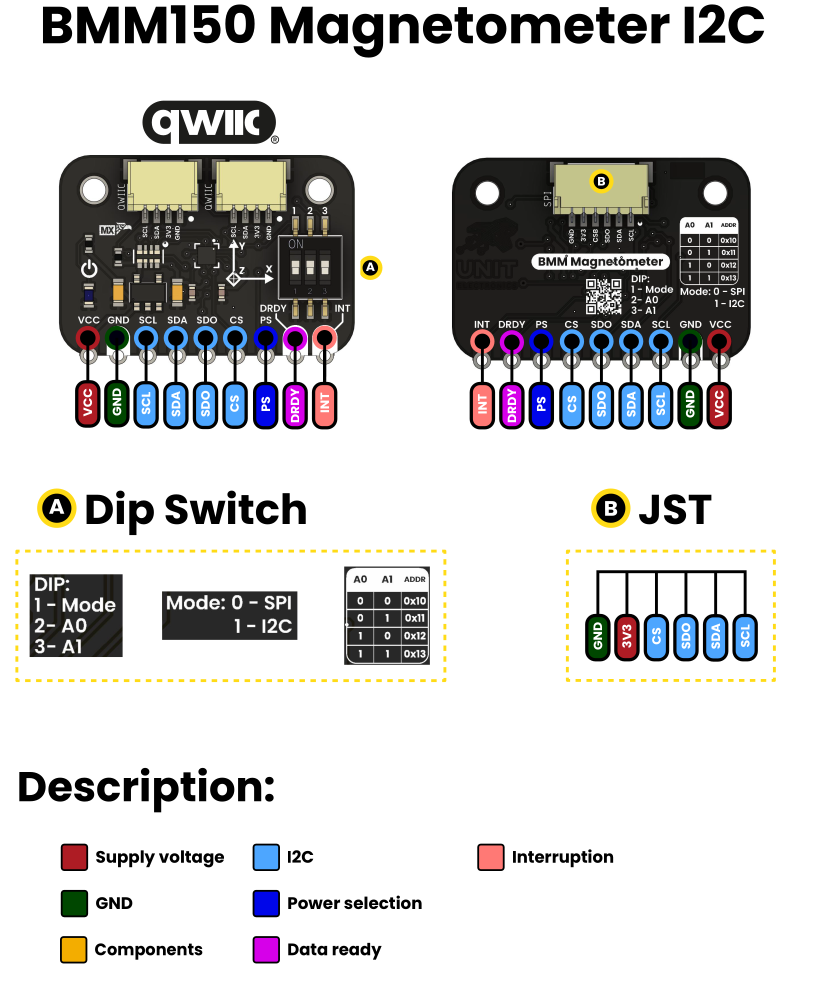
\includegraphics[width=0.95\textwidth,keepaspectratio]{images/function-diagram.png}
\end{center}
\newpage
\vspace*{3em}
\section*{Dimensions}
\vspace{1em}
\begin{center}
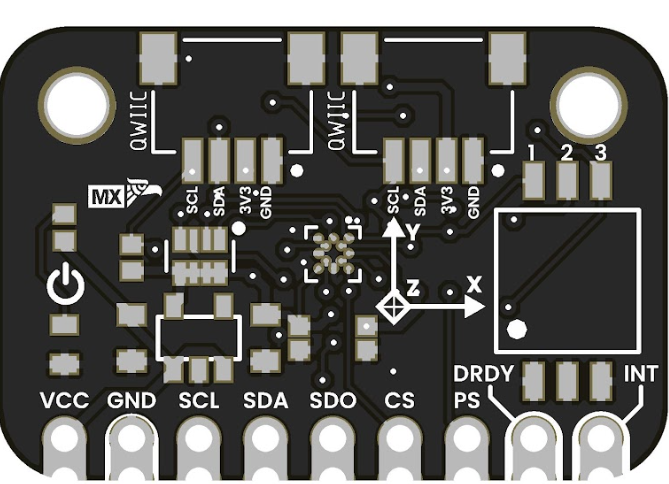
\includegraphics[width=0.95\textwidth,keepaspectratio]{images/dimensions.png}
\end{center}



% Uso
\section*{Usage}
\begin{itemize}
\item Arduino AVR
\item Raspberry Pi RP2040
\item ESP32
\end{itemize}

% Descargas
\section*{Downloads}
\begin{itemize}
\begin{itemize}
\item \href{../hardware/}{Schematic PDF}
\end{itemize}
\end{itemize}

% Compra
\section*{Purchase}
\begin{itemize}
\item \href{https://www.uelectronics.com}{Buy from UNIT Electronics}
\end{itemize}

\end{document}
